%Master File:lectures.tex

\lesson{Know Your Graph Algorithms}

\vspace{-2cm}
\begin{center}
  \includegraphics[height=10cm]{mst_full}%\pause
%  \llap{\includegraphics[height=10cm]{rednose}}\pauseb
\end{center}
\keywords{Weighted graph algorithms, Minimum spanning tree, Prim, Kruskal, shortest path, Dijkstra}\pauselevel{=1}\pause

%%%%%%%%%%%%%%%%%%%%%%% Next Slide %%%%%%%%%%%%%%%%%%%%%%%
\renewcommand{\Outline}{%
\begin{slide}
\section[1]{Outline}

\begin{minipage}{12cm}
  \begin{enumerate}\squeeze
    \outlineitem{Minimum Spanning Tree}{mstqq}
    \outlineitem{Prim's Algorithm}{primqq}
    \outlineitem{Kruskal's Algorithm}{kruskalqq}
    \outlineitem{Union Find}{unionfind}
    \outlineitem{Shortest Path}{dijkstraqq}
  \end{enumerate}
\end{minipage}\hfill
\begin{minipage}{10cm}
  \includegraphics[width=10cm]{mst_full}
\end{minipage}
\end{slide}
\addtocounter{outlineitem}{1}
}

\setcounter{outlineitem}{1}
\Outline
\toptarget{firstoutline}
%%%%%%%%%%%%%%%%%%%%%%% Next Slide %%%%%%%%%%%%%%%%%%%%%%%

\begin{slide}
\section{Graph Algorithms}

\begin{PauseHighLight}
  \begin{itemize}
  \item We consider a graph algorithm to be \emph{efficient} if it can
    solve a graph problem in $O(n^a)$ time for some fixed $a$\pause
  \item That is, an efficient algorithm runs in polynomial time\pause
  \item A problem is \emph{hard} if there is no known efficient
    algorithm\pause
  \item This does \emph{not} mean the best we can do is to look through
    all possible solutions---see later lectures\pause
  \item In this lecture we are going to look at some efficient graph
  algorithms for weighted graphs\pause
  \end{itemize}
\end{PauseHighLight}

\end{slide}

%%%%%%%%%%%%%%%%%%%%%%% Next Slide %%%%%%%%%%%%%%%%%%%%%%%

\begin{slide}
\section[-2]{Minimum spanning tree}

\pausebuild
\color{TwoColor}
\begin{itemize}
\item  A minimal spanning tree is the shortest tree which spans the
  entire graph\pause
  \vspace*{-1cm}
  \begin{center}\pauselevel{=1, :2}\color{TextColor}
    \multiinclude[graphics={height=13cm}]{PrimGraph}\pause
  \end{center}
  \vspace*{-1cm}
\end{itemize}
\end{slide}

%%%%%%%%%%%%%%%%%%%%%%% Next Slide %%%%%%%%%%%%%%%%%%%%%%%

\begin{slide}
\section{Greedy Strategy}

\begin{PauseHighLight}
  \begin{itemize}
  \item We consider two algorithms for solving the problem
    \begin{itemize}
    \item \toplink{prim}{Prim's algorithm} (discovered 1957)
    \item \toplink{kruskal}{Kruskal's algorithm} (discovered 1956)\pause
    \end{itemize}
  \item Both algorithms use a \emph{greedy strategy}\pause
  \item Generally greedy strategies are not guaranteed to give
    globally optimal solutions\pause
  \item There exists a class of problems with a \emph{matroid}
    structure where greedy algorithms lead to globally optimal
    solutions\pause
  \item Minimum spanning trees, Huffman codes and shortest path
    problems are matroids\pause
  \end{itemize}
\end{PauseHighLight}

\end{slide}


%%%%%%%%%%%%%%%%%%%%%%% Next Slide %%%%%%%%%%%%%%%%%%%%%%%
\Outline % Prim's
%%%%%%%%%%%%%%%%%%%%%%% Next Slide %%%%%%%%%%%%%%%%%%%%%%%

\begin{slide}
\section[-2]{Prim's Algorithm}
\toptarget{prim}

\pausebuild
\color{TwoColor}
\begin{itemize}\squeeze
\item Prim's algorithm grows a subtree greedily\pauseh
\item Start at an arbitrary node\pauseh
\item Add the shortest edge to a node not in the tree
  \pauselevel{=1, highlight =3 :10}\pause
\end{itemize}
  \vspace*{-1cm}
  \begin{center}\pauselevel{=1, :2}\color{TextColor}
    \multiinclude[graphics={height=11cm}]{Prim}\pause
  \end{center}
  \vspace*{-1cm}
\end{slide}


%%%%%%%%%%%%%%%%%%%%%%% Next Slide %%%%%%%%%%%%%%%%%%%%%%%

\begin{slide}
\section[-2.4]{Pseudo Code}

\begin{pseudo}
#\textsc{Prim}#($G=(\mathcal{V},\mathcal{E},\bm{w})$)$\pauseh$ {
   for i:=1 to $|\mathcal{V}|$
      $d_i$ := $\infty$               \\ Minimum 'distance' to subtree
   endfor$\pauseh$
   $\mathcal{E}_T\,$ := $\,\emptyset$                  \\ Set of edges in subtree
   PQ.initialise()       \\ initialise an empty priority queue
   node := $\,\,v_1$              \\ where $v_1\in\mathcal{V}\,\,$ is arbitrary$\pauseh$
   for i:=1 to $|\mathcal{V}|-1$
      $d_{\mathtt{node}}$ := 0$\pauseh$
      for k $\in \{v\in\mathcal{V}| (\mathtt{node},v)\in\mathcal{E}\}$ \\ $\mathtt{k}\ $ is a neighbours of $\mathtt{node}$
         if ( $w_{\mathtt{node,k}} < d_{\mathtt{k}}\,\,$  )
            $d_{k}$ := $w_{\mathtt{node,k}}$
            PQ.add( ($d_{\mathtt{k}}$, (node,k)) )
         endif
      endfor$\pauseh$
      do
         (a_node, next_node) := PQ.getMin()
      until ($d_{\mathtt{next\_node}}$  > 0)$\pauseh$
      $\mathcal{E}_T$ := $\mathcal{E}_T \cup \{($a_node, next_node)$\}$
      node := next_node$\pauseh$
   endfor
   return $\mathcal{E}_T$
}$\pauseh$
\end{pseudo}
\vspace*{-1cm}
\end{slide}

%%%%%%%%%%%%%%%%%%%%%%% Next Slide %%%%%%%%%%%%%%%%%%%%%%%

\begin{slide}
\section[-2]{Prim's Algorithm in Detail}
\pb
\pause
\begin{center}
  \includegraphics[width=0.9\linewidth]{prim-0}\mypl{1}
  \multido{\ia=1+1,\ib=2+1}{22}%
  {\llap{\includegraphics[width=0.9\linewidth]{prim-\ia}\mypl{\ib}}}
\end{center}
\end{slide}


%%%%%%%%%%%%%%%%%%%%%%% Next Slide %%%%%%%%%%%%%%%%%%%%%%%

\begin{slide}
\section{Why Does This Work?}

\begin{PauseHighLight}
  \begin{itemize}
  \item Clearly Prim's algorithm produces a spanning tree\pause
    \begin{itemize}
    \item It is a tree because we always choose an edge to a node not in
      the tree\pause
    \item It is a spanning tree because it has $|\mathcal{V}|-1$ edges\pause
    \end{itemize}
  \item Why is this a minimum spanning tree?\pause
  \item Once again we look for a proof by induction\pause
  \end{itemize}
\end{PauseHighLight}

\end{slide}

%%%%%%%%%%%%%%%%%%%%%%% Next Slide %%%%%%%%%%%%%%%%%%%%%%%

\begin{slide}
\section[-1]{Proof by induction}

\begin{PauseHighLight}
  \begin{itemize}
  \item We want to show that each subtree, $T_i$, for $i=1, 2, \cdots, n$ is
    part of (a subgraph) of some minimum spanning tree\pause
  \item In the base case, $T_1$ consists of a tree with no edges,
    but this has to be part of the minimum spanning tree\pause
  \item To prove the inductive case we assume that $T_i$ is part of the
    minimum spanning tree\pause
  \item We want to prove that $T_{i+1}$ formed by adding the shortest
    edge is also part of the minimum spanning tree\pause
  \item We perform the proof by contradiction\pause---we assume that
    this added edge isn't part of the minimum spanning tree\pause
  \end{itemize}
\end{PauseHighLight}

\end{slide}

%%%%%%%%%%%%%%%%%%%%%%% Next Slide %%%%%%%%%%%%%%%%%%%%%%%

\begin{slide}
\section[-2]{Contrariwise}
\pb
\pause

\begin{center}
  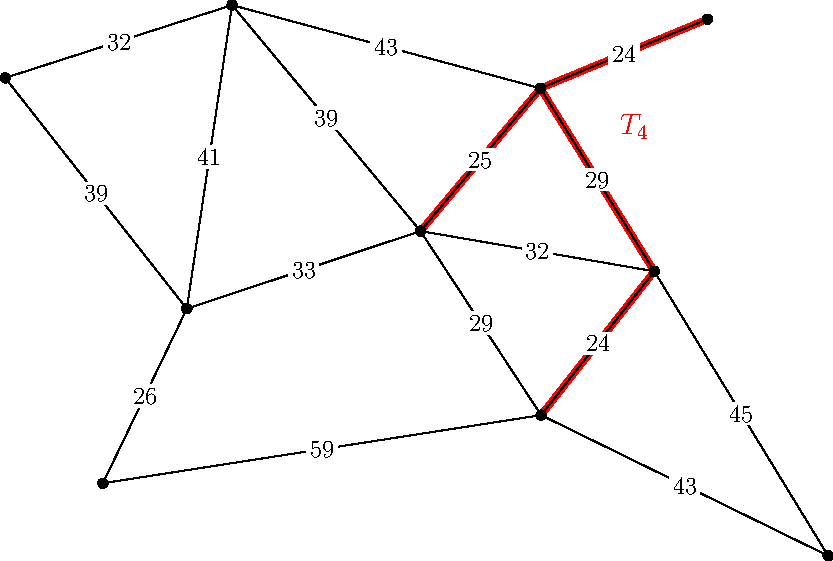
\includegraphics[height=12cm]{prim_proof0}\mypl{1}
  \multido{\ia=1+1,\ib=2+1}{3}%
  {\llap{\includegraphics[height=12cm]{prim_proof\ia}\mypl{\ib}}}
\end{center}


\end{slide}

%%%%%%%%%%%%%%%%%%%%%%% Next Slide %%%%%%%%%%%%%%%%%%%%%%%

\begin{slide}
\section[-2.4]{Loop Counting}

\begin{pseudo}
#\textsc{Prim}#($G=(\mathcal{V},\mathcal{E}, \bm{w})$) {
   for i:=0 to $|\mathcal{V}|$
      $d_i$ := $\infty$ 
   endfor
   $\mathcal{E}_T\,$ := $\,\emptyset$
   PQ.initialise()
   node := $\,\,v_1$
   for i:=1 to $|\mathcal{V}|-1$                            // loop 1  $O(|\mathcal{V}|)$
      $d_{node}$ := 0
      for k $\in \{v\in\mathcal{V}| (\mathtt{node},v)\in\mathcal{E}\}$                       // inner loop $O(|\mathcal{E}|/|\mathcal{V}|)$
         if ( $w_{node,k} < d_{k}\,\,$  )
            $d_{k}$ := $w_{node,k}$
            PQ.add( ($d_{k}$, (node,k)) )              // $O\bigl(\log(|\mathcal{E}|)\bigr)$
         endif
      endfor
      do
         (a_node, next_node) := PQ.getMin()
      until ($d_{next\_node}$  > 0)
      $\mathcal{E}_T$ := $\mathcal{E}_T \cup \{($node, next_node)$\}$
      node := next_node
   endfor
   return $\mathcal{E}_T$
}
\end{pseudo}
\vspace*{-1cm}
\end{slide}

%%%%%%%%%%%%%%%%%%%%%%% Next Slide %%%%%%%%%%%%%%%%%%%%%%%

\begin{slide}
\section{Run Time}

\begin{PauseHighLight}
  \begin{itemize}
  \item The worst time is
    \begin{align*}
      O(|\mathcal{V}|) \times
      O\left(\frac{|\mathcal{E}|}{|\mathcal{V}|}\right) \times
      O\bigl(\log(|\mathcal{E}|)\bigr)\pause = O\left(\strut
      |\mathcal{E}|\log(|\mathcal{E}|)\right)\pause
    \end{align*}
    \item Note that  $|\mathcal{E}| < |\mathcal{V}|^2$\pause
    \item Thus, $\log(|\mathcal{E}|) <
       2 \log(|\mathcal{V}|) = O\left(\strut
        \log(|\mathcal{V}|) \right)$\pause
    \item Thus the worst case time complexity is $|\mathcal{E}|
    \log(|\mathcal{V}|)$\pause
  \end{itemize}
\end{PauseHighLight}

\end{slide}


%%%%%%%%%%%%%%%%%%%%%%% Next Slide %%%%%%%%%%%%%%%%%%%%%%%
\Outline % Kruskal's
%%%%%%%%%%%%%%%%%%%%%%% Next Slide %%%%%%%%%%%%%%%%%%%%%%%

\begin{slide}
\section[-2]{Kruskal's Algorithm}
\toptarget{kruskal}

\pausebuild
\color{TwoColor}
\begin{itemize}\squeeze
\item Kruskal's algorithm works by choosing the shortest edges which
  don't form a loop\pause
\end{itemize}
  \vspace*{-1cm}
  \begin{center}\pauselevel{=1, :2}\color{TextColor}
    \multiinclude[graphics={height=13cm}]{Kruskal}\pause
  \end{center}
  \vspace*{-1cm}
\end{slide}

%%%%%%%%%%%%%%%%%%%%%%% Next Slide %%%%%%%%%%%%%%%%%%%%%%%

\begin{slide}
\section[-1]{Pseudo Code}

\begin{pseudo}
#\textsc{Kruskal}#($G=(\mathcal{V},\mathcal{E}, \bm{w})$)$\pauseh$
{
   PQ.initialise()
   for edge  $\in |\mathcal{E}|$
      PQ.add( ($w_{edge}$, edge) )
   endfor$\pauseh$

   $\mathcal{E}_T\,$ := $\,\emptyset$
   noEdgesAccepted := 0$\pauseh$

   while (noEdgesAccepted < $|\mathcal{V}|-1$)
      edge := PQ.getMin()
      if $\mathcal{E}_T \cup \{$edge$\}$ is acyclic
         $\mathcal{E}_T$ := $\mathcal{E}_T \cup \{$edge$\}$
         noEdgesAccepted := noEdgesAccepted +1
      endif
   endwhile$\pauseh$

   return $\mathcal{E}_T$
}$\pauseh$
\end{pseudo}
\vspace*{-1cm}
\end{slide}

%%%%%%%%%%%%%%%%%%%%%%% Next Slide %%%%%%%%%%%%%%%%%%%%%%%

\begin{slide}
\section{Analysis}

\begin{PauseHighLight}
  \begin{itemize}
  \item Kruskal's algorithm looks much simpler than Prim's\pause
  \item The sorting takes most of the time, thus Prim's algorithms is
    $O\bigl(|\mathcal{E}| \log(|\mathcal{E}|)\bigr) = O\bigl(|\mathcal{E}|
    \log(|\mathcal{V}|)\bigr)$\pause
  \item We can sort the edges however we want---we could use quick sort
    rather than heap sort using a priority queue\pause
  \item But we haven't specified how we determine if the added edge
    would produce a cycle\pause
  \end{itemize}
\end{PauseHighLight}

\end{slide}

%%%%%%%%%%%%%%%%%%%%%%% Next Slide %%%%%%%%%%%%%%%%%%%%%%%

\begin{slide}
\section[-1]{Cycling}

\begin{PauseHighLight}
  \begin{itemize}
  \item For a path to be a cycle the edge has to join two nodes
    representing the same subtree\pause
  \item To compute this we need to quickly \emph{find} which subtree a
    node has been assigned to\pause
  \item Initially all nodes are assigned to a separate subtree\pause
  \item When two subtrees are combined by an edge we have to perform the
    \emph{union} of the two subtrees\pause
  \item This is a tricky but standard operation known as
    \emph{union-find}\pause
  \end{itemize}
\end{PauseHighLight}

\end{slide}

%%%%%%%%%%%%%%%%%%%%%%% Next Slide %%%%%%%%%%%%%%%%%%%%%%%
\Outline % Union-Find
%%%%%%%%%%%%%%%%%%%%%%% Next Slide %%%%%%%%%%%%%%%%%%%%%%%

\begin{slide}
\section{Union-Find}

\begin{PauseHighLight}
  \begin{itemize}
  \item In the union-find algorithm we have a set of objects $x \in 
    \mathcal{S}$ which are to be grouped into subsets $\mathcal{S}_1$,
    $\mathcal{S}_2$, \ldots\pause
  \item Initially each object is in its individual subset (no relationships)\pause
  \item We want to make the \emph{union} of two subsets (add
    relationship between elements)\pause
  \item We also want to \emph{find} the subset given an element\pause
  \item This is a common problem for which we will write a class
  \jl$DisjointSets$ to perform fast \texttt{union}s and \texttt{find}s\pause
  \end{itemize}
\end{PauseHighLight}

\end{slide}

%%%%%%%%%%%%%%%%%%%%%%% Next Slide %%%%%%%%%%%%%%%%%%%%%%%

\begin{slide}
\section[-1]{DisjointSets}

\begin{PauseHighLight}
  \begin{itemize}
  \item We want to create a class
    \begin{java}
class DisjointSets
{
    DisjointSets(int numElements) {/* Constructor */}
    int find(int x) {/* Find root */}
    void union(int root1, int root2) {/* Union */}

    private:
      int[] s;
}$\pause$
    \end{java}
  \item Where \jl$find(x)$ returns a unique identifier for the subset
    which element \jl$x$ belongs to\pause
  \item The array \jl$s$ contains labelling information to implement
    \jl$find(x)$\pause
  \end{itemize}
\end{PauseHighLight}

\end{slide}

%%%%%%%%%%%%%%%%%%%%%%% Next Slide %%%%%%%%%%%%%%%%%%%%%%%

\begin{slide}
\section[-1]{The Union-Find Dilemma}

\begin{PauseHighLight}
  \begin{itemize}
  \item A natural algorithm to perform finds is to maintain an
    array returning a subset label for each element\pause---this makes
    \texttt{find} fast\pause
  \item However, every time we combine two subset we have to change all
    the labels in this array (taking $O(n)$ operations)\pause
  \item If we are unlucky the cost of performing $n$ unions is
    $\Theta(n^2)$\pause
  \item If we ensure that we relabel the smaller subset then the time
    complexity is $\Theta(n \log(n))$\pause
  \item Fast \textit{finds} seems to give slow(ish) \textit{unions}\pause
  \item What about the other way around?\pause
  \end{itemize}
\end{PauseHighLight}

\end{slide}

%%%%%%%%%%%%%%%%%%%%%%% Next Slide %%%%%%%%%%%%%%%%%%%%%%%

\begin{slide}
\section{Fast Union}

\begin{PauseHighLight}
  \begin{itemize}
  \item To achieve fast unions we can represent our disjoint sets as a
    forest (many disjoint trees)\pause
  \item Every time we perform a union we make one of the trees point to
    the head of the other tree\pause
  \item The cost of \texttt{find} depends on the depth of the tree\pause
  \item To make unions efficient we make the shallow tree a subtree of
    the deeper tree\pause
  \end{itemize}
\end{PauseHighLight}

\end{slide}


%%%%%%%%%%%%%%%%%%%%%%% Next Slide %%%%%%%%%%%%%%%%%%%%%%%

\begin{slide}
\section[-2]{Putting it Together}
\pb

\begin{center}
  \multiinclude[graphics={height=14cm}]{disjointset}\pause
\end{center}

\end{slide}

%%%%%%%%%%%%%%%%%%%%%%% Next Slide %%%%%%%%%%%%%%%%%%%%%%%

\begin{slide}
\section[-2]{Smart Union}

\begin{PauseHighLight}
\begin{java}
    DisjointSets::DisjointSets(int numElements)
    {
        s = new int[numElements];
        for(int i=0; i<s.length; i++)
            s[i] = -1;                   // roots are negative number
    }$\pause$

    void DisjointSets::union(int root1, int root2)
    {
        if (s[root2]<s[root1]) {         // root2 is deeper
            s[root1] = root2;            // make root2 the root$\pause$
        } else {
            if (s[root1]==s[root2])      
                s[root1]--;              // update height if same
            s[root2] = root1;            // make root1 new root
        }
    }$\pause$
\end{java}
\begin{center}
  \includegraphics[width=0.9\linewidth]{disjointDiag}
\end{center}
\end{PauseHighLight}
\end{slide}

%%%%%%%%%%%%%%%%%%%%%%% Next Slide %%%%%%%%%%%%%%%%%%%%%%%

\begin{slide}
\section{Path Compression}

\begin{PauseHighLight}
  \begin{itemize}
  \item To speed up \texttt{find} we relabel all nodes we visit during
    \texttt{find} by the root label\pause
    \begin{java}
    public int DisjointSets::find(int index)
    {
        if (s[index]<0)
            return index;
        else
            return s[index] = find(s[index]);
    }$\pause$
    \end{java}
  \end{itemize}
  \begin{center}
    \includegraphics[width=0.9\linewidth]{disjointDiag1}
  \end{center}
\end{PauseHighLight}

\end{slide}

%%%%%%%%%%%%%%%%%%%%%%% Next Slide %%%%%%%%%%%%%%%%%%%%%%%

\begin{slide}
\section[-1]{Mazes}

\pb
\begin{minipage}{15cm}
  \begin{itemize}\squeeze
  \item Union-Find is a data structure which can occur in very different
    applications\pauseh
  \item One application is building a maze\pauseh
  \item Start from a complete lattice\pauseh
  \item Remove a randomly chosen edge if it connects two unconnected
    regions\pauseh
  \item Stop when the start and end cell are connected\pauseh
  \item Or better after all cells are connected\pauseh
  \end{itemize}
\end{minipage}\hfill
\begin{minipage}{8cm}
  \begin{picture}(80,150)
    \put(0,0){\includegraphics[width=8cm]{maze.0}}
    \pauselevel{=1}\pause
    \put(0,0){\includegraphics[width=8cm]{maze.1}}
    \pauselevel{=4}\pause
    \put(0,0){\includegraphics[width=8cm]{maze.2}}
    \pauselevel{=5}\pause
    \put(0,0){\includegraphics[width=8cm]{maze.3}}
    \pauselevel{=6}\pause
  \end{picture}
\end{minipage}
\end{slide}


%%%%%%%%%%%%%%%%%%%%%%% Next Slide %%%%%%%%%%%%%%%%%%%%%%%

\begin{slide}
\section{Time Complexity of Union-Find}

\pb
\begin{itemize}
\item If we perform $M$ finds and $N$ unions then the time complexity
  is $O\bigl(M\log_2^*(N)\bigr)$\pauseh
\item Where $\log_2^*(N)$ is the number of times you need to apply the
  logarithm function before you get a number less than 1\pauseh
\item In practice $\log_2^*(N)\leq 5$ for all conceivable $N$\pauseh
  \begin{align*}
    \hspace{3cm}\log_2(10^{80}) = 265.75 \mypl{4}
    \mathllap{\log_2(\log_2(10^{80})) = 8.0539\mypl{5}}
    \mathllap{\log_2(\log_2(\log_2(10^{80}))) = 3.0097\mypl{6}}
    \mathllap{\log_2(\log_2(\log_2(\log_2(10^{80})))) = 1.5896\mypl{7}}
    \mathllap{\log_2(\log_2(\log_2(\log_2(\log_2(10^{80}))))) = 0.66868\pause}
  \end{align*}
\item The proof of this time complexity is rather involved\pause
\end{itemize}

\end{slide}


%%%%%%%%%%%%%%%%%%%%%%% Next Slide %%%%%%%%%%%%%%%%%%%%%%%
\Outline % Dijkstra
%%%%%%%%%%%%%%%%%%%%%%% Next Slide %%%%%%%%%%%%%%%%%%%%%%%



\begin{slide}
\section[-1]{Shortest path}

\begin{PauseHighLight}
  \begin{itemize}
  \item We can efficiently compute the shortest path from one vertex to
    any other vertex\pause
  \item This defines a spanning tree, but where the optimisation
    criteria is that we choose the vertex that are closest to the
    \textit{source}\pause
  \item To find this spanning tree we use Dijkstra's algorithm where we
    successively add the nearest node to the source which is connected
    to the subtree built so far\pause
  \item This is very close to Prim's algorithm and has the same
    complexity\pause
  \end{itemize}
\end{PauseHighLight}

\end{slide}
%%%%%%%%%%%%%%%%%%%%%%% Next Slide %%%%%%%%%%%%%%%%%%%%%%%

\begin{slide}
\section[-2]{Dijkstra's Algorithm}

\pb
\begin{center}
  \multiinclude[graphics={height=14cm}]{Dijkstra}\pause
\end{center}
\end{slide}

%%%%%%%%%%%%%%%%%%%%%%% Next Slide %%%%%%%%%%%%%%%%%%%%%%%

\begin{slide}
\section[-2.4]{Pseudo Code}

\begin{pseudo}
#\textsc{Dijkstra}#($G=(\mathcal{V},\mathcal{E},\bm{w})$, source)$\pauseh$ {
   for i:=0 to $|\mathcal{V}|$
      $d_i$ := $\infty$               \\ Minimum 'distance' to source
   endfor$\pauseh$
   $\mathcal{E}_T\,$ := $\,\emptyset$                  \\ Set of edges in subtree
   PQ.initialise()       \\ initialise an empty priority queue
   node := source              $\pauseh$
   $d_{node}$ := 0$\pauseh$
   for i:=1 to $|\mathcal{V}|-1$
      for k $\in \{v\in\mathcal{V}| (\mathtt{node},v)\in\mathcal{E}\}$ 
         if ( $w_{node,k}+d_{node} < d_{k}\,\,$  )
            $d_{k}$ := $w_{node,k}+d_{node}$
            PQ.add( ($d_{k}$, (node, k)) )
         endif
      endfor$\pauseh$
      do
         (a_node, next_node) := PQ.getMin()
      while next_node not in subtree$\pauseh$
      $\mathcal{E}_T$ := $\mathcal{E}_T \cup \{($a_node, next_node)$\}$
      node := next_node$\pauseh$
   endfor
   return $\mathcal{E}_T$
}$\pauseh$
\end{pseudo}
\vspace*{-1cm}

\end{slide}
%%%%%%%%%%%%%%%%%%%%%%% Next Slide %%%%%%%%%%%%%%%%%%%%%%%

\begin{slide}
\section[-2.4]{Compare to Prim's Algorithm}

\begin{pseudo}
#\textsc{Prim}#($G=(\mathcal{V},\mathcal{E},\bm{w})$) {
   for i:=1 to $|\mathcal{V}|$
      $d_i$ := $\infty$               \\ Minimum 'distance' to subtree
   endfor
   $\mathcal{E}_T\,$ := $\,\emptyset$                  \\ Set of edges in subtree
   PQ.initialise()       \\ initialise an empty priority queue
   node := $\,\,v_1$              \\ where $v_1\in\mathcal{V}\,\,$ is arbitrary
   for i:=1 to $|\mathcal{V}|-1$
      $d_{\mathtt{node}}$ := 0$\pauseh$
      for k $\in \{v\in\mathcal{V}| (\mathtt{node},v)\in\mathcal{E}\}$
         if ( $w_{\mathtt{node,k}} < d_{\mathtt{k}}\,\,$  )
            $d_{k}$ := $w_{\mathtt{node,k}}$
            PQ.add( ($d_{\mathtt{k}}$, (node,k)) )
         endif
      endfor
      do
         (a_node, next_node) := PQ.getMin()
      until ($d_{\mathtt{next\_node}}$  > 0)
      $\mathcal{E}_T$ := $\mathcal{E}_T \cup \{($a_node, next_node)$\}$
      node := next_node
   endfor
   return $\mathcal{E}_T$
}
\end{pseudo}
\vspace*{-1cm}
\end{slide}

%%%%%%%%%%%%%%%%%%%%%%% Next Slide %%%%%%%%%%%%%%%%%%%%%%%

\begin{slide}
\section{Dijkstra Details}

\begin{PauseHighLight}
  \begin{itemize}
  \item Dijkstra is very similar to Prim's (it differs in the distances
    that are used)\pause
  \item It has the same time complexity\pause
  \item It can be viewed as using a greedy strategy\pause
  \item It can also be viewed as using the dynamic programming strategy
    (see lecture 22)\pause
  \end{itemize}
\end{PauseHighLight}

\end{slide}

%%%%%%%%%%%%%%%%%%%%%%% Next Slide %%%%%%%%%%%%%%%%%%%%%%%

\begin{slide}
\section{Lessons}

\begin{PauseHighLight}
  \begin{itemize}
  \item There are many efficient (i.e. polynomial $O(n^a)$) graph
    algorithms\pause
  \item Some of the most efficient ones are based on the Greedy
    strategy\pause
  \item These are easily implemented using priority queues\pause
  \item Minimum spanning trees are useful because they are easy to
    compute\pause
  \item Dijkstra's algorithm is one of the classics\pause
  \end{itemize}
\end{PauseHighLight}

\end{slide}
